%Standalone output. Only use size of content for the pdf.
\documentclass{standalone} 

%Scalable font similar to cm.
\usepackage{lmodern} 
 
 

%############################################
%Colors and images.
%############################################

%Importing images.
\usepackage{graphicx} 

%More colors.
\usepackage[dvipsnames]{xcolor} 

%Colored frames in equations.
\usepackage{empheq}

%Tikz/pgf package to program graphics.
\usepackage{tikz} 

%Some useful libraries. Babel to fix problems with babel package.
\usetikzlibrary{positioning, calc, intersections, cd, babel} 
\usepackage{tikz-3dplot}


%############################################
%Tables and lists.
%############################################

%Colors in tables.
\usepackage{colortbl} 

%Long tables that allows page breaks.
\usepackage{longtable} 

%Join cells in a row.
%\multicolumn{n}{cols}{text} already included. \multirow{n}{width, * for default size}{text} is added by the package.
\usepackage{multirow} 





%############################################
%Mathematics.
%############################################

%Standard mathematics.
\usepackage{amsmath,amsthm,amsfonts,amssymb,mathtools} 

%\mathbbm{1} for unity operator.
\usepackage{bbm} 

%\nicefrac{}{} and units.
\usepackage{units} 

%Crossing out in formulas with \cancel{expression}.
\usepackage{cancel} 

%Tensor indices
\usepackage{tensor} 

%Fixes space around \ldots.
\usepackage{ellipsis}

%Bold mathematics in headings, etc..
\makeatletter
\g@addto@macro\bfseries{\boldmath}
\makeatother
	
%Notation quantum mechanics.
\newcommand{\bra}[1]{\langle #1 |}
\newcommand{\ket}[1]{| #1 \rangle}
\newcommand{\braket}[1]{\langle #1 \rangle}
\newcommand{\Bra}[1]{\left\langle #1 \right|}
\newcommand{\Ket}[1]{\left| #1 \right\rangle}
\newcommand{\Braket}[1]{\left\langle #1 \right\rangle}

%\boxed with additional horizontal space.
\newcommand{\widebox}[1]{\boxed{\hspace{1em}#1\hspace{1em}}}






\begin{document}
	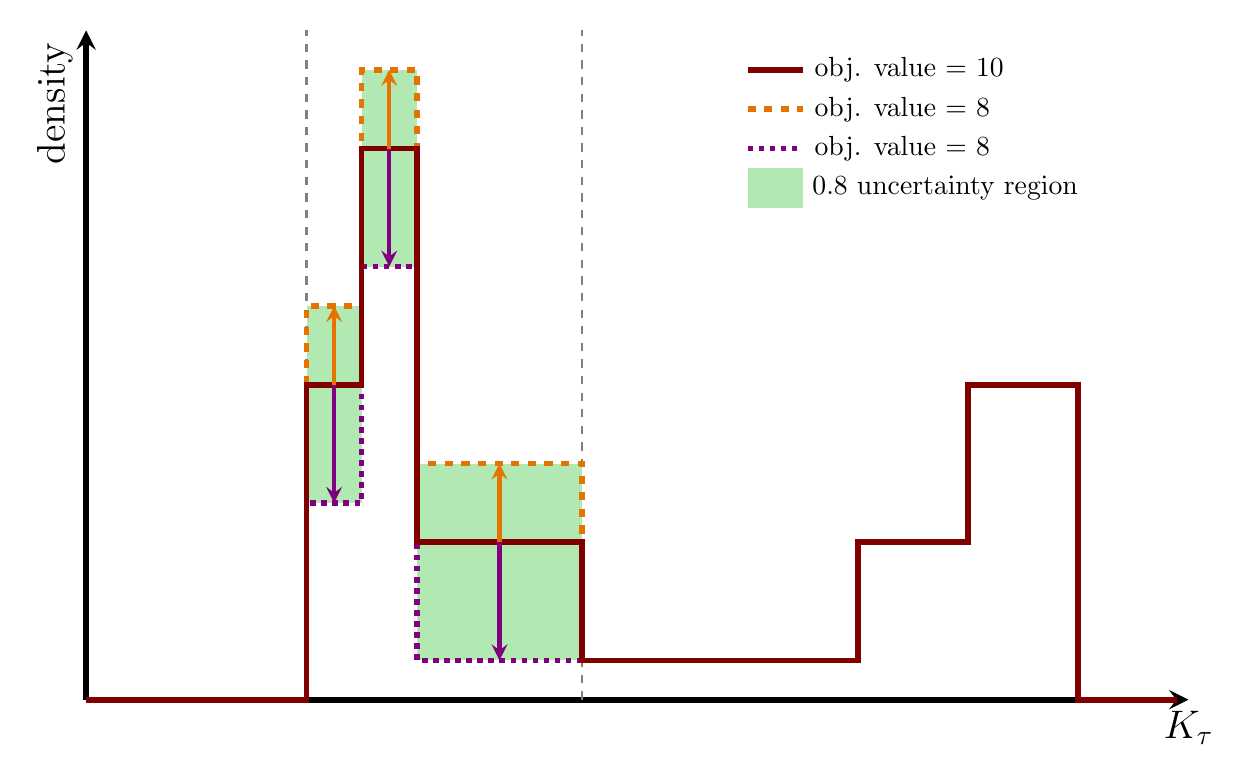
\begin{tikzpicture}[xscale = 1.4]
		\draw[-stealth, line width = 2pt] (0,0) --  (10,0) node[below]{\Large$K_\tau$};
		\draw[-stealth, line width = 2pt] (0,0) --  (0,8.5) node[left = 0.4cm, rotate=90]{\Large density};

		\fill[green!70!black!30] (2,2.5) rectangle (2.5,5);
		\fill[green!70!black!30] (2.5,5.5) rectangle (3,8);
		\fill[green!70!black!30] (3,0.5) rectangle (4.5,3);

		\draw[black!50, thick, dashed] (2,0)--(2,8.5);
		\draw[black!50, thick, dashed] (4.5,0)--(4.5,8.5);

		\draw[orange!90!black, line width = 2pt, dashed] (2,4) -- (2,5) -- (2.5,5)--(2.5,8)--(3,8)--(3,3)--(4.5,3)--(4.5,2);

		\draw[blue!50!red, line width = 2pt, dotted] (2,4) -- (2,2.5) -- (2.5,2.5)--(2.5,5.5)--(3,5.5)--(3,0.5)--(4.5,0.5)--(4.5,2);


		\draw[red!50!black, line width = 2pt] (0,0) --(2,0)--(2,4)--(2.5,4) -- (2.5,7) --(3,7)--(3,2)--(4.5,2)--(4.5,0.5)--(7,0.5)--(7,2)--(8,2)--(8,4)--(9,4)--(9,0)--(9.9,0);
		
		\draw[red!50!black, line width = 2pt] (6,8)--(6.5,8) node[black, right]{obj. value = 10};
		\draw[orange!90!black, line width = 2pt, dashed] (6,7.5)--(6.5,7.5) node[black, right]{obj. value = 8};
		\draw[blue!50!red, line width = 2pt, dotted] (6,7)--(6.5,7) node[black, right]{obj. value = 8};

		\draw[green!70!black!30] (6,6.5)--(6.5,6.5) node[black, right]{0.8 uncertainty region};
		\fill[green!70!black!30] (6,6.25) rectangle (6.5,6.75);


		\draw[orange!90!black, line width = 1.5pt, -stealth] (2.25,4)--(2.25,5);
		\draw[orange!90!black, line width = 1.5pt, -stealth] (2.75,7)--(2.75,8);
		\draw[orange!90!black, line width = 1.5pt, -stealth] (3.75,2)--(3.75,3);

		\draw[blue!50!red, line width = 1.5pt, -stealth] (2.25,4)--(2.25,2.5);
		\draw[blue!50!red, line width = 1.5pt, -stealth] (2.75,7)--(2.75,5.5);
		\draw[blue!50!red, line width = 1.5pt, -stealth] (3.75,2)--(3.75,0.5);

	\end{tikzpicture}
\end{document}
